\documentclass{beamer}
% \documentclass[handout]{beamer}
\usepackage{pgfpages}
\setbeameroption{show notes on second screen}
% \pgfpagesuselayout{2 on 1}[a4paper,border shrink=10mm]

\usepackage{ccicons}
\usepackage{fontawesome}
\usepackage{hyperref}
\usepackage{minted}


% ❤️ https://github.com/elauksap/focus-beamertheme
\usetheme{focus}
\title{Reactive Applications\\in Frontend Engineering Today}
\author{Manuel Alabor}
\institute{Master Seminar\\HSR University of Applied Sciences Rapperswil}
\date{}

\setminted{autogobble=true, tabsize=2, linenos=false, frame=none, breaklines=true}

\begin{document}

\begin{frame}
	\maketitle
	\Tiny{\ccby\thinspace\thinspace This work is licensed under a \href{https://creativecommons.org/licenses/by/4.0/}{Creative Commons Attribution 4.0 International License}}.
\end{frame}

\note[itemize]{
	\item Welcome To My Talk
}

\section*{Welcome}

\begin{frame}{Motivation and Goals}
	\begin{itemize}
		\item Get \textbf{acquainted} with \textbf{scientific research work style}\bigskip
		\item \textbf{Review} a research report\bigskip
		\item \textbf{Transfer} topic to the \textbf{field} of \textbf{frontend engineering}\bigskip
		\item \textbf{Write} a research report\bigskip
	\end{itemize}
\end{frame}

\note[itemize]{
	\item This was my first seminar paper done
	\item Given goals summarized:
	\item Learn scientific work style
	\item Review report, write an own afterwards
	\item Transfer a topic to another area (frontend engineering)\bigskip
	\item To do so, Markus came up with an interesting paper:
}

\begin{frame}[focus]
	\emph{``On the Positive Effect of Reactive Programming on Software Comprehension: An Empirical Study''}
	\\\bigskip
	\small{Salvaneschi et al. \cite{7827078}}
\end{frame}

\note[itemize]{
	\item On the positive effect of reactive programming on software comprehension
	\item An empirical study
	\item Research Group around Guido Salvaneschi
}

\subsection*{Research Questions}

\begin{frame}{RQ1: Design Sciences and \\Empirical Software Engineering}
	\begin{enumerate}
		\item[RQ1.1] Which \textbf{empirical research methods}, approaches and concepts \textbf{were applied} by Salvaneschi et al. \cite{7827078}?\bigskip
		\item[RQ1.2] Are these research methods, approaches and concepts \textbf{applied well}, what could have been done better?\bigskip
		\item[RQ1.3] \textbf{Do} Salvaneschi et al. \cite{7827078} \textbf{meet FAIR principles} \cite{2019arXiv190805986H} \cite{wilkinson:2016} with their work?
	\end{enumerate}
\end{frame}

\note[itemize]{
	\item Our own goals are formalized by a total of 7 research Questions
	\item The first set investigates in how well Salvaneschi et al. did their work:
	\item Which empirical research methods, approaches and concepts were applied
	\item Are these research methods, approaches and concepts applied well, what could have been done better?
	\item Do they meet FAIR principles?
}

\begin{frame}{RQ2: Software Engineering Principles}
	\begin{itemize}
		\item[RQ2.1] \textbf{How} do Salvaneschi et al. \cite{7827078} \textbf{define RP and OOP}?\bigskip
		\item[RQ2.2] \textbf{When} should \textbf{RP be considered}, and \textbf{when not}?\bigskip
		\item[RQ2.3] \textbf{Which experiments} should be \textbf{conducted in future} work?\bigskip
		\item[RQ2.4] \textbf{Which} design \textbf{alternatives exist} in the context of \textbf{frontend engineering}?
	\end{itemize}
\end{frame}

\note[itemize]{
	\item The second set looks on the following questions related to software engineering:
	\item How does the group define RP and OOP?
	\item When should RP be applied, and when not?
	\item Where could a future research project continue?
}

\section{Summary of Salvaneschi et al.}

\note[itemize]{
	\item Lets begin now with the main part
	\item See what Salvaneschi and his reserarch group worked on...
}

\begin{frame}[focus]
	``\emph{(...) it has been repeatedly argued that RP greatly improves (...) comprehension of software.}''
	\\\bigskip
	\small{Salvaneschi et al. \cite{7827078}}
\end{frame}

\note[itemize]{
	\item This is the main thesis of Salvaneschi et al
	\item They build four research questions:
}

\begin{frame}{Research Questions \cite{7827078}}
	\begin{itemize}
		\item \emph{``Does reactive programming \textbf{impact the correctness} of program comprehension?''}\bigskip
		\item \emph{``Does reactive programming \textbf{impact time} for program comprehension?''}\bigskip
		\item \emph{``Does comprehending RP programs \textbf{require a different programming skills level} than the OO style?''}\bigskip
		\item \emph{``What are the \textbf{reasons for a difference} - if any - in comprehending RP programs and OO programs?''}
	\end{itemize}
\end{frame}

\note[itemize]{
	\item Does RP have an impact on how correct a program is comprehended?
	\item Are there differences in how much time is required to comprehend an RP program?
	\item Does RP need a higher or lower skill level to correctly understand a programs source code?
	\item Can we reason why there are differences between comprehending OOP and RP code?\bigskip
	\item What did they do?
	\begin{itemize}
		\item The group set up a controlled experiment
		\item Total of 127 students participated
		\item Preparatory skill level survey (quantitative)
		\item Additional Quantitative and qualitative survey to capture personal opinion afterwards
	\end{itemize}
}

\subsection*{Study Results}
\begin{frame}{Study Results}
	\begin{block}{Finding 1: \textbf{Correctness}}
		RP \textbf{increases} the \textbf{correctness} of program \textbf{comprehension}
	\end{block}
	\begin{block}{Finding 2: \textbf{Time}}
		RP style code \textbf{does not} require \textbf{more time} than comprehending its OOP equivalent
	\end{block}
	\begin{block}{Finding 3: \textbf{Skill Level}}
		RP code is \textbf{easier to understand} overall, \textbf{regardless} of the individuals programming \textbf{skill level}
	\end{block}
\end{frame}

\note[itemize]{
	\item Their work resulted in, along others, three main findings:
	\begin{itemize}
		\item \textbf{Correctness}: RP code was better to understand than its OOP equivalent
		\item \textbf{Time}: RP code did not require more time to understand
		\item \textbf{Skill level}: Overall, RP code was easier to understand, regardless of the individuals personal programming skill level
	\end{itemize}
}


\section{Review of Salvaneschi et al.}
\note[itemize]{
	\item Back to our own research questions
	\item I will present you two score cards
	\item One card per question set
	\item Each giving an overview how well Salvaneshi et al worked in the respective area
}


\subsection*{Research Principle Score Card}
\begin{frame}{Research Principle Score Card}
	\begin{exampleblock}{\faicon{thumbs-o-up} Empirical Software Engineering}
		\begin{itemize}
			\item \textbf{Careful} study \textbf{setup} and \textbf{execution}
			\item \textbf{Transparent} description of \textbf{threats to validity}
		\end{itemize}
	\end{exampleblock}

	\begin{alertblock}{\faicon{thumbs-o-down} Design Sciences}
		\textbf{No evidence} for the \textbf{application} of \textbf{design sciences} found
	\end{alertblock}

	\begin{alertblock}{\faicon{thumbs-o-down} FAIR Research Principles}
		Lack of \textbf{complementary information} violates \textbf{Reusability} principle
	\end{alertblock}
\end{frame}

\note[itemize]{
	\item \textbf{Empirical Software Engineering}: Well done, nothing to complain\bigskip
	\item \textbf{Design Sciences}: No clear evidence for use
	\item This is one study of many... Did they use Design Sciences for their high level planning?\bigskip
	\item \textbf{FAIR}: Good, except: Complementary information is missing
	\item Survey Tool and full code samples would improve value significantly
}


\subsection*{Software Engineering Score Card}
\begin{frame}{Software Engineering Score Card}
	\begin{exampleblock}{\faicon{thumbs-o-up} Reactive Applications}
		Introduction of classification schema: \textbf{Synthetic} and \textbf{interactive} applications, \textbf{graphical animations}
	\end{exampleblock}
	\begin{exampleblock}{\faicon{thumbs-o-up} Reactive Programming}
		\begin{itemize}
			\item Good overview noting \textbf{origins} in FP and \textbf{recent} development
			\item \textbf{Examples} using Scala
		\end{itemize}
	\end{exampleblock}

	\begin{alertblock}{\faicon{thumbs-o-down} Object Oriented Programming}
		\begin{itemize}
			\item \textbf{Limited overview} compared to RP
			\item \textbf{Reduced} to Observer Pattern, still \textbf{used synonymously}
		\end{itemize}
	\end{alertblock}
\end{frame}

\note[itemize]{
	\item \textbf{Reactice Applications}: Introduction of classification schema\bigskip
	\item \textbf{Reactive Programming}: Good introduction to the subject
	\item Good examples in Scala using REScala\bigskip
	\item \textbf{OOP}: Short introduction compared to RP.
	\item Sad: Reduced to observer pattern, used as synonym throughout the work
}


\section{Application in Frontend Engineering}
\note[itemize]{
	\item Classification system introduced by Salvaneschi et al
	\item Transfer to two own examples
	\item We left out "graphical animation" by intention
	\item (Efficient) Animations in frontends usually done using CSS animations
}


\subsection*{Synthetic Application}
\begin{frame}{Synthetic Application: Scenario}
	\begin{columns}
		\column{0.6\textwidth}
			\begin{itemize}
				\item \textbf{Fetch} and \textbf{combine remote} profile and avatar \textbf{resource}\bigskip
				\item Avatar \textbf{depends} on profile resource\bigskip
			\end{itemize}

		\column{0.4\textwidth}
			\begin{block}{S1: \textbf{Modelling Data Flow}}
				\textbf{Fetch} a users \textbf{complete} profile \textbf{information} (name as well as their avatar picture) from \textbf{two} distinct \textbf{data sources}. The \textbf{profile} information \textbf{contains} required input to fetch the \textbf{avatar}. \textbf{Show} the combined information in the user interface \textbf{at once}.
			\end{block}
	\end{columns}
\end{frame}

\note[itemize]{
	\item Scenario: Show a users profile information with avatar
	\item Fetch an combine two remote data sources
	\item To fetch avatar, profile is required to be present
	\item This is a synthetic application: Model data flow
	\item With reactive programming, this looks like:
}

\begin{frame}[fragile=singleslide]{Synthetic Application: Reactive Programming}
	\begin{block}{Modelling Data Flow with Promises}
		\begin{minted}{JavaScript}
			fetchProfile()
				.then(async (profile) => {
					const avatar = await fetchAvatar(profile);
					return { ...profile, ...avatar };
				})
				.then(renderUser);
		\end{minted}
	\end{block}
\end{frame}

\note[itemize]{
	\item Using Promises, this is straighforward
}

\begin{frame}[fragile=singleslide]{Synthetic Application: Observer Pattern}
	\begin{block}{Modelling Data Flow with Observer Design Pattern \cite{gamma1995design} I}
		\begin{minted}{JavaScript}
			const profileObservable = observable();
			const avatarObservable = observable();
		\end{minted}
	\end{block}
\end{frame}

\note[itemize]{
	\item With an Observer after Gamma et al
	\item Start with the definition of two observables for profile and avatar
}

\begin{frame}[fragile=singleslide]{Synthetic Application: Observer Pattern}
	\begin{block}{Modelling Data Flow with Observer Design Pattern \cite{gamma1995design} II}
		\begin{minted}{JavaScript}
			profileObservable.addObserver(async () => {
				const avatar = await fetchAvatar(profileObservable.value);
				avatarObservable.value = avatar;
				avatarObservable.notify();
			});

			avatarObservable.addObserver(() => {
				renderUser({
					...profileObservable.value,
					...avatarObservable.value
				});
			});
		\end{minted}
	\end{block}
\end{frame}

\note[itemize]{
	\item Define behavior for each observable
	\item What happens when profile arrives?
	\item What happens when avatar arrives?
}

\begin{frame}[fragile=singleslide]{Synthetic Application: Observer Pattern}
	\begin{block}{Modelling Data Flow with Observer Design Pattern \cite{gamma1995design} III}
		\begin{minted}{JavaScript}
			fetchProfile().then(profile => {
				profileObservable.value = profile;
				profileObservable.notify();
			});
		\end{minted}
	\end{block}
\end{frame}

\note[itemize]{
	\item Finally kick code into action
	\item Fetch profile and notify observers
}

\begin{frame}{Synthetic Application: Key Findings}
	\begin{itemize}
		\item \textbf{Key findings} in favor of reactive programming by Salvaneschi et al. \cite{7827078} \textbf{confirmed}:\smallskip
		\begin{itemize}
			\item \textbf{Less boilerplate} code\smallskip
			\item \textbf{Mental model} can be implemented \textbf{more accurately}
		\end{itemize}\bigskip
		\item \textbf{Reactive programming} is \textbf{better} suited for the implementation of \textbf{synthetic applications}
	\end{itemize}
\end{frame}

\note[itemize]{
	\item You might already guess\dots
	\item We verified key finding by Salvaneschi et al
	\item RP requires less boilerplate code
	\item Mental model more or less 1 to 1 in code
	\item At least for syntehtic applications
}

\subsection*{Interactive Application}
\begin{frame}[t]{Interactive Application}
	\begin{columns}[t]
		\column{0.5\textwidth}
			\begin{itemize}
				\item \textbf{Handle} user \textbf{interaction} with a user interface \textbf{component}
			\end{itemize}

		\column{0.5\textwidth}
			\begin{block}{S2: \textbf{Handle User Interaction}}
				Handle clicks on a button. \textbf{Every time} a \textbf{user clicks} the \textbf{button}, \textbf{log} the current \textbf{time}. The log shows a list of all user interactions eventually.
			\end{block}
	\end{columns}
\end{frame}

\note[itemize]{
	\item Second scenario rather simple
	\item React on clicks on a button
	\item Trigger an action accordinlgy
	\item Here: Log the current date and time in a log
}

\begin{frame}[fragile=singleslide]{Interactive Application: Reactive Programming}
	\begin{block}{Handle User Interaction with BaconJS}
		\begin{minted}{JavaScript}
			Bacon.fromEvent(getButton(), "click")
				.map(() => new Date())
				.onValue(logInteraction);
		\end{minted}
	\end{block}
\end{frame}

\note[itemize]{
	\item Reactive Programming
	\item BaconJS runtime
	\item Hook up to button click events
	\item Get current time in a map combinator
	\item Pass time in onValue side effect
}

\begin{frame}[fragile=singleslide]{Interactive Application: Observer Pattern}
	\begin{block}{Handle User Interaction with EventTarget Interface}
		\begin{minted}{JavaScript}
			getButton().addEventListener(
				"click",
				() => logInteraction(new Date())
			);
		\end{minted}
	\end{block}
\end{frame}

\note[itemize]{
	\item Buttons implement the DOMs EventTarget interface
	\item Register an observer to the buttons click events
}

\begin{frame}{Interactive Application: Key Findings}
	\begin{itemize}
		\item \textbf{Both} solutions have similar \textbf{small code footprint}\bigskip
		\item \textbf{Reactive programming} variation introduces \textbf{hidden complexity}\bigskip
		\item \textbf{Do not use} any paradigm simply \textbf{for the sake of it}
	\end{itemize}
\end{frame}

\note[itemize]{
	\item Not much different using RP or observers
	\item Why? EventTarget DOM API is already observer based
	\item Even worse: Hidden complexity through RP runtime
	\item Use the right tool for the right thing (TM)
}

\subsection*{Criteria Catalog}
\begin{frame}[focus]
	When Should I\\Use What?!
\end{frame}

\note[itemize]{
	\item Unsatisfying outcome
	\item No recipe
	\item If A then RP, else Observer
	\item What can we do?
	\item We dont know
	\item But we might give a good starting point when evaluating between RP and the observer
}

\begin{frame}[fragile=singleslide]{Criteria Catalog}
	\begin{figure}
		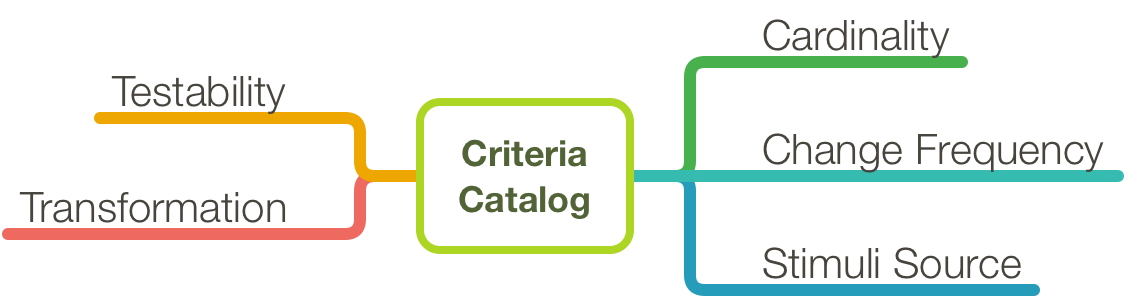
\includegraphics[width=\textwidth]{assets/slides/criteria-catalog.png}
	\end{figure}
\end{frame}

\note[itemize]{
	\item Interesting Questions to ask:
	\item \textbf{Cardinality}: How many components consume values?
	\item \textbf{Change Frequency}: How many values are expected to be emitted over time?
	\item \textbf{Stimuli Source}: Where do values come from? A remote data source? Triggered by users? What APIs are available for these sources? What about fail tolerance?
	\item \textbf{Testability}: What test methods do you want to apply? Blackbox? Break down larger components?
	\item \textbf{Transformation}: Do you need to combine values from multiple sources? How are these combined? How do you need to transform them?
}

\section{Outlook}
\begin{frame}{Future Research Suggestions}
	\begin{enumerate}
		\item \textbf{Verify} presented \textbf{scenarios} and \textbf{criteria catalog} in an empirical study\bigskip
		\item \textbf{Explore W3C Web Animation API} draft for more complex, high-performance animation behaviors\bigskip
		\item Research to \textbf{improve} development \textbf{tool support} for \textbf{reactive programming}
	\end{enumerate}
\end{frame}

\note[itemize]{
	\item How could future research invest?\bigskip
	\item \textbf{Empirical Study}: Verify presented two scenarios and criteria catalog
	\item Yield valuable output for projects facing a decision\bigskip
	\item \textbf{Explore} in W3C Web Animation API: RP meets efficient browser animations\bigskip
	\item As suggested by Salvaneschi et al: Research in improving RP \textbf{tool support} (Debugging, IDEs)
}

\section{Conclusion}
\begin{frame}{Recap}
	\begin{itemize}
		\item \textbf{Summary and review} on paper by Salvaneschi et al. \cite{7827078}\bigskip
		\item \textbf{Transferred} results by Salvaneschi et al. \textbf{to} context of \textbf{frontend engineering}\bigskip
		\item \textbf{Suggested three} potential \textbf{topics} for future research
	\end{itemize}
\end{frame}

\note[itemize]{
	\item We showed:
	\item Summary and review
	\item Transferred to Frontend Engineeringh
	\item Suggested Three Follow Up Topics for Future Research
}

\begin{frame}
	\begin{center}
		\emph{We selected ``Research to improve development tool support for reactive programming'' as topic for our own future research.}
	\end{center}
\end{frame}

\begin{frame}[focus]
	Questions?
\end{frame}

\begin{frame}[focus]
	Discussion
\end{frame}

\appendix
\begin{frame}[allowframebreaks]{References}
	\bibliographystyle{plain}
	\bibliography{bibliography}
\end{frame}

\end{document}